In den nachfolgenden Abschnitten werden die Erweiterungen von MMFGs und deren Voraussetzungen vorgestellt und detailliert beschrieben.

Die Struktur dieser Abschnitte folgt der logischen aufeinander aufbauenden Reihenfolge der Erweiterungen von einfachen MMFGs über SMMFGs zu ESMMFGs.
In \cref{sec2:sota:par:basic-formal-representation-mmfgs} werden die formalen Grundlagen der beschriebenen Erweiterungen vorgestellt und detailliert erläutert.
In \cref{sec2:sota:par:annot-formal-representation-mmfgs} werden Annotierungen von MMFGs eingeführt, auf deren Basis in \cref{sec2:sota:par:semantic-annot-formal-representation-smmfgs} semantische Erweiterungen in Form von SMMFGs aufbauen.
Schlussendlich führt das Anwenden einer Phrasenstruktur-Grammatik in \cref{sec2:sota:par:explainable-smmfgs} zu ESMMFGs.

\paragraph{Grundlagen der formalen Darstellung von MMFGs}
\label{sec2:sota:par:basic-formal-representation-mmfgs}
Die Datenstruktur der MMFGs bietet selbst keine Funktionalitäten und ist eine simple generische Datenstruktur zur Abbildung identifizierter Merkmale und deren Beziehungen zueinander in Form von Knoten und Kanten.
Um eine formale Darstellung von MMFGs durch eine formale Sprache zu erreichen, kann eine Grammatik angewendet werden. 
Eine Grammatik $G$ für eine Sprache $L$ ist definiert durch ein Quadrupel $G = (N,~\Sigma,~P,~S)$:
\begin{enumerate}
    \setlength{\itemsep}{0pt}
    \item $N$ ist eine endliche, nichtleere Menge von \textit{Nichtterminalen}.
    \item $\Sigma$ ist eine endliche, nichtleere Menge von \textit{Terminalen}, welche zulässige Sätze der Sprache $L$ abschließen. Die endlichen, nichtleeren Mengen $N$ und $\Sigma$ sind disjunkt, $N \cap \Sigma = \varnothing$.
    \item $P \subseteq N \times (N \cup \Sigma)^{*}$ ist eine Menge von \textit{Produktionsregeln}.
    \item $S \in N$ ist das Startsymbol.
\end{enumerate}
Damit die Struktur der MMFGs die formale Darstellung durch eine Grammatik unterstützt, muss die Struktur der MMFGs durch ein zusätzliches Element $S_{MMFG}$ erweitert werden.
Dieses zusätzliche Element $S_{MMFG}$ dient als Startsymbol für zulässige formale Ausdrücke der Sprache $L$.
Die Erweiterung eines MMFGs durch ein solches Startsymbol ist in \cref{sec2:sota:subsec:fz-explainablity:fig:mmfg-add-start} zu sehen. 
Hier und in den weiteren Abschnitten werden diese Formen der Erweiterungen anhand des $MMFG_{ex}$ aus \cref{sec2:sota:subsec:fz-explainablity:fig:mmfg-example} demonstriert.

%\begin{figure}[htb]
    \centering
    \resizebox{\textwidth}{!}{
        \begin{tikzpicture}[font=\fontsize{9}{0pt}\selectfont]

            \definecolor{e4draw}{RGB}{224,155,254}
            \definecolor{n5fill}{RGB}{84,224,163}
            \definecolor{node}{RGB}{51, 175, 255}
            \definecolor{compr}{RGB}{224, 155, 254}
            \definecolor{sr}{RGB}{84, 224, 163}

            \tikzset{
                e1/.style={-{Triangle[angle=90:3pt,length=1.5mm,fill=black]}},
                e2/.style={-{Triangle[angle=90:3pt,length=1.5mm,fill=e4draw]}},
                e3/.style={-{Triangle[angle=90:3pt,length=1.5mm,fill=n5fill]}},
                comprstyle/.style={-{Triangle[angle=90:3pt,length=1.5mm,fill=compr]}},
                srstyle/.style={-{Triangle[angle=90:3pt,length=1.5mm,fill=sr]}},
                thick/.style={line width=1.1pt},
                every node/.append style={thick}
            }

            \node[draw, minimum width=\textwidth, minimum height=3.8cm] (f) {};

            \node[anchor=north west] at (f.north west) {(a)};
            \node[anchor=north east] at (f.north east) {(b)};

            \node[anchor=south west, rectangle, draw, line width=0.4pt] at (f.south west) {%
                \shortstack[l]{Erweiterung eines MMFG \\um Wurzelknoten $S_{MMFG}$}
            };

            \node[anchor=south east, rectangle, draw, line width=0.4pt] at (f.south east) {%
                \shortstack[l]{Formales Schema der Darstellung \\des $MMFG_{ex}$}
            };

            \draw[] ([xshift=4.3cm]f.north west) -- ([xshift=4.3cm]f.south west);

            \node[rectangle, draw, anchor=north west, fill=orange] (smmfg) at ([xshift=1cm, yshift=-0.7cm]f.north west) {$S_{MMFG}$};

            \node[rectangle, draw, fill=node, right=2.3cm of smmfg] (person) {\textit{\textbf{n: Person}}};
            \node[rectangle, draw, fill=node, below=0.7cm of person] (body) {\textit{\textbf{n: Body}}};
            \node[rectangle, draw, fill=node, right=1cm of body] (arm) {\textit{\textbf{n: Arm}}};
            \node[rectangle, draw, fill=compr, above=0.7cm of arm] (att) {\textit{\textbf{attached to}}};
            \node[rectangle, draw, fill=node, right=1cm of arm] (watch) {\textit{\textbf{n: Watch}}};
            \node[rectangle, draw, fill=sr, right=1cm of watch] (clock) {\textit{\textbf{s: Clock}}};
            

            \draw[e1] (smmfg.east) -- node[below] {\textit{\textbf{cn}}} (person.west);
            \draw[e1] (person.south) -- node[left] {\textit{\textbf{cn}}} (body.north);
            \draw[e1] (body.east) -- node[above] {\textit{\textbf{cn}}} (arm.west);
            \draw[comprstyle, draw=compr] (att.south) -- node[left] {\textit{\textbf{cr}}} (arm.north);
            \draw[comprstyle, draw=compr] (watch.north) |- node[right] {\textit{\textbf{cr}}} (att.east);
            \draw[e1] (arm.east) -- node[above] {\textit{\textbf{cn}}} (watch.west);
            \draw[srstyle, draw=sr] (watch.east) -- node[above] {\textit{\textbf{sr}}} (clock.west);

        \end{tikzpicture}
    }
    \caption{(\textbf{a}) Erweiterung des $MMFG_{ex}$ um ein Startsymbol $S_{MMFG}$, (\textbf{b}) Formales Schema der Darstellung des $MMFG_{ex}$.}
    \label{sec2:sota:subsec:fz-explainablity:fig:mmfg-add-start}
\end{figure}
\begin{figure}[htb]
    \centering
    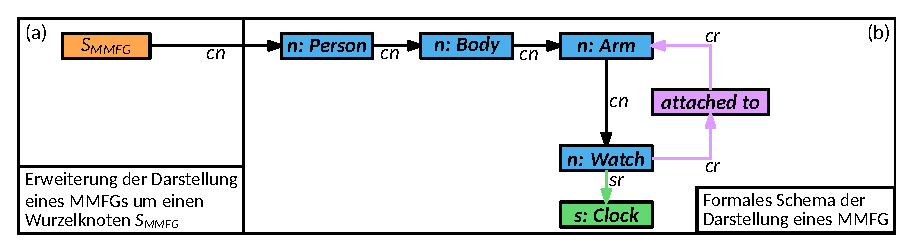
\includegraphics[width=\textwidth]{chapter/chapter_2/mmfg/formal/formal-schema-mmfg-ex.eps}
    \caption{(\textbf{a}) Erweiterung des $MMFG_{ex}$ um ein Startsymbol $S_{MMFG}$, (\textbf{b}) Formales Schema der Darstellung des $MMFG_{ex}$.}
    \label{sec2:sota:subsec:fz-explainablity:fig:mmfg-add-start}
\end{figure}

Eine grundlegende Grammatik $G_{MMFG} = (N_{MMFG},~\Sigma_{MMFG},~P_{MMFG},~S_{MMFG})$ zur Konstruktion zulässiger formaler Ausdrücke aus einem MMFG lautet wie folgt:
\begin{itemize}
    \item $N_{MMFG} = FVT_{MMFG}~\cup~FRT_{MMFG}$.
    $FVT_{MMFG} = \{fvt_{1},...,fvt_{n}\}$ ist der Wortschatz der Merkmale eines MMFG und stellt die Bezeichnungen der identifizierten Merkmale dar.
    $FRT_{MMFG}$ stellt die Beziehungstypen zwischen Merkmalen in einem MMFG dar.
    \item $\Sigma_{MMFG}$ ist die Menge textueller Beschreibungen ($LBL$) für Elemente aus den Mengen $FVT_{MMFG}$ und $FRT_{MMFG}$.
    \item $P_{MMFG}$ ist die Menge an Produktionsregeln, welche zulässige Sätze anhand der Mengen $FVT_{MMFG}$ und $FRT_{MMFG}$ bildet.
    Eine einfache Form von Produktionsregeln kann wie folgt definiert werden:
    \newlength{\s}
    \setlength{\s}{\widthof{$S_{MMFG} \hspace*{\widthof{$FVT_{MMFG}$} - \widthof{$S_{MMFG}$}}\rightarrow FVT_{MMFG}~FRT_{MMFG}~FVT_{MMFG}$}}
    \newlength{\p}
    \setlength{\p}{\widthof{$P_{MMFG} = \{$}}
    \begin{align*}
        %\begin{split}
            P_{MMFG} = \{ \hspace*{\s + 0.1cm} \\
            S_{MMFG} \hspace*{\widthof{$FVT_{MMFG}$} - \widthof{$S_{MMFG}$}}\rightarrow FVT_{MMFG}~FRT_{MMFG}~FVT_{MMFG} \\
            FVT_{MMFG} \rightarrow LBL \hspace*{\s - \widthof{$FVT_{MMFG} \rightarrow LBL$}} \\
            FRT_{MMFG} \rightarrow LBL \hspace*{\s - \widthof{$FRT_{MMFG} \rightarrow LBL$}} \\
            \} \hspace{\s}
        %\end{split}
    \end{align*}
    \item $S_{MMFG}$ ist der Wurzelknoten des MMFG.
\end{itemize}
Eine Anwendung der Grammatik $G_{MMFG}$ auf den $MMFG_{ex}$ aus \cref{sec2:sota:subsec:fz-explainablity:fig:mmfg-add-start} führt zu formalen Ausdrücken wie \enquote{body has-child arm. arm has-child watch. watch is-attached-to arm}.
Aufgrund der Produktionsregel $S_{MMFG}$ in $G_{MMFG}$ weisen alle mit dieser Grammatik generierten Ausdrücke das Muster \textit{Knoten-Kante-Knoten} auf.

Durch das Erweitern eines MMFG mit einem Startsymbol, sowie das Anwenden einer Grammatik können bereits grundlegende formale Darstellungen von MMFGs erreicht werden.
Die formale Modellierung einer solchen formalen Darstellung eines MMFGs ist in \cref{sec2:sota:subsec:fz-explainablity:fig:mmfg-formal-model} zu sehen.

%\begin{figure}[htb]
    \centering
    \resizebox{\textwidth}{!}{
        \begin{tikzpicture}[font=\fontsize{9}{0pt}\selectfont]

            \definecolor{e4draw}{RGB}{224,155,254}
            \definecolor{n5fill}{RGB}{84,224,163}
            \definecolor{node}{RGB}{51, 175, 255}
            \definecolor{compr}{RGB}{224, 155, 254}
            \definecolor{sr}{RGB}{84, 224, 163}

            \tikzset{
                e1/.style={-{Triangle[angle=90:3pt,length=1.5mm,fill=black]}},
                e2/.style={-{Triangle[angle=90:3pt,length=1.5mm,fill=e4draw]}},
                e3/.style={-{Triangle[angle=90:3pt,length=1.5mm,fill=n5fill]}},
                comprstyle/.style={-{Triangle[angle=90:3pt,length=1.5mm,fill=compr]}},
                srstyle/.style={-{Triangle[angle=90:3pt,length=1.5mm,fill=sr]}},
                thick/.style={line width=1.1pt},
                every node/.append style={thick}
            }

            \node[text width=2.5cm] (formal-model) at (0,0) {
                \shortstack{Formale \\Modellierung \\der Darstellung \\eines MMFG}
            };

            \node[anchor=south west, text width=2.5cm] (anchor-annot) at (formal-model.north west) {
                \shortstack{Anker von \\Annotierungen}
            };

            \tikzmath{
                coordinate \p;
                \p = (formal-model.south west) - (anchor-annot.north west);
                \len = veclen(\p);
            }

            \node[anchor=south east, minimum height=\len] (mmfg) at (formal-model.south west) {
                \hspace*{1mm}
                \begin{turn}{90}
                    \fontsize{12}{0}\fontseries{bx}\selectfont
                    MMFG
                \end{turn}
                \hspace*{1mm}
            };

            \tikzmath{
                coordinate \mmfg;
                \mmfg = (mmfg.south west) - (mmfg.south east);
                \mmfglen = veclen(\mmfg);
            }

            \node[draw, rectangle, fit={(mmfg)($(mmfg.south east)+(\textwidth,0)$)}, style={inner sep=0pt}] (f) {};

            \tikzmath{
                coordinate \f;
                \f = (f.south east) - (formal-model.south east);
                \flen = veclen(\f) * 0.0352778;
            }

            \draw[line width=1.1pt] (mmfg.north east) -- (mmfg.south east);
            \draw[] (anchor-annot.north east) -- (formal-model.south east);
            \draw[] (formal-model.north west) -- (formal-model.north east); 

            \path[name path=f-eastl] (f.north east) -- (f.south east);
            \path[name path=div1] (formal-model.north east) -- ++(\flen,0);
            \path[name intersections={of=div1 and f-eastl, by=div-f}];

            \draw[] (formal-model.north east) -- (div-f);





            \node[rectangle, draw, fill=node, right=1.5cm of formal-model.east, text width=2cm, align=center] (fvt1) {$S_{MMFG}$};
            \node[rectangle, draw, fill=node, right=1cm of fvt1, text width=2cm, align=center] (fvt2) {$fvt$};
            \node[rectangle, draw, fill=node, right=1cm of fvt2, text width=2cm, align=center] (fvt3) {$fvt$};

            \draw[e1] (fvt1.east) -- node[below] {$frt$} (fvt2.west);
            \draw[e1] (fvt2.east) -- node[below] {$frt$} (fvt3.west);

            \foreach \x in {0,...,4} {
                \node[rectangle, draw, right=1cm + 2.33cm * \x of anchor-annot.east, line width=0.4pt] (aa-\x) {$LBL$};
            }

            \draw[e1] (fvt1.north) -- (aa-0.south);
            \draw[e1] (fvt1.east) ++(5mm,0cm) -- (aa-1.south);
            \draw[e1] (fvt2.north) -- (aa-2.south);
            \draw[e1] (fvt2.east) ++(5mm,0cm) -- (aa-3.south);
            \draw[e1] (fvt3.north) -- (aa-4.south);

        \end{tikzpicture}
    }
    \caption{Formale Modellierung der Darstellung eines MMFGs.}
    \label{sec2:sota:subsec:fz-explainablity:fig:mmfg-formal-model}
\end{figure}
\begin{figure}[htb]
    \centering
    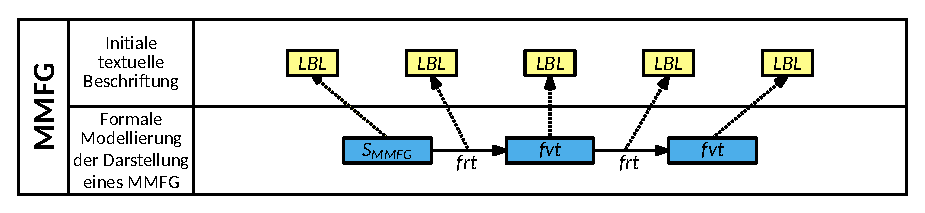
\includegraphics[width=\textwidth]{chapter/chapter_2/mmfg/formal/formal-model-syntactic-mmfg.eps}
    \caption{Formale Modellierung der Darstellung eines MMFGs.}
    \label{sec2:sota:subsec:fz-explainablity:fig:mmfg-formal-model}
\end{figure}

Auch wenn mit dieser Grammatik bereits eine grundlegende formale Darstellung von MMFGs möglich ist, verbleiben noch eine Reihe offener Herausforderungen in Bezug auf die Grammatik:
\begin{itemize}
    \item Die Grammatik $G_{MMFG}$ stellt nicht die Struktur von MMFGs dar.
    \item Die Grammatik $G_{MMFG}$ ist keine kontextfreie Grammatik.
    \item Die Grammatik $G_{MMFG}$ spiegelt nicht die Struktur der Elemente in einem MMFG, sowie die dafür notwendigen Produktionsregeln wieder.
    So sollte die Kindsbeziehung (cn) zwischen den Knoten \textit{Person} und \textit{Body} in $MMFG_{ex}$ durch den Text \enquote{has a child named} repräsentiert werden.
    \item Die Grammatik $G_{MMFG}$ bietet keine semantische Beschreibung der zwischen Merkmalen bestehenden Beziehungen.
\end{itemize}
Zusammenfassend werden weitere Erweiterungen, vor allem in Bezug auf höhere semantische Darstellungen und verbesserte Lesbarkeit, benötigt.
Basierend auf der in diesem Abschnitt demonstrierten Erweiterungen werden in den nächsten Abschnitten semantische und erklärbare MMFGs (SMMFGs bzw. ESMMFGs) modelliert.
Hierzu werden in den nächsten Abschnitt mehrere Erweiterungen von MMFGs, sowie entsprechende Grammatiken beschrieben. 

\paragraph{Annotation der formalen Darstellung von MMFGs}
\label{sec2:sota:par:annot-formal-representation-mmfgs}
Höhere semantische Darstellungen bzw. Beschriftungen können durch das Anbinden von externen Informationssystemen, wie z.B. dem Semantic Web oder WikiData erreicht werden.
Das Anbinden solcher externen Informationssysteme wird durch das Hinzufügen eines neuen Knotens, einem sogenannten Anker für Annotationen (engl. \textit{annotation anchor $(aa)$}), in die Darstellung von MMFGs ermöglicht.
Diese Anker für Annotationen können über eine ebenfalls neu hinzugefügte Beziehung, der Beziehung für Annotationen (engl. \textit{annotation relationship $(ar)$}), mit Knoten oder Kanten des MMFGs verbunden werden.
Durch das Hinzufügen der beiden neuen Elemente können nun Knoten, sowie auch Kanten mit diesen neuen Elementen verbunden werden.
Auf diese Weise kann jedes Element in einem MMFG semantisch annotiert werden.
Die formale Darstellung eines MMFG mitsamt Annotationsanker ist in \cref{sec2:sota:subsec:fz-explainablity:fig:mmfg-formal-model-mmfg-incl-annotations} abgebildet und wird in den folgenden Abschnitten als Grundlage für weitere Erweiterungen dienen.

\begin{figure}[htb]
    \centering
    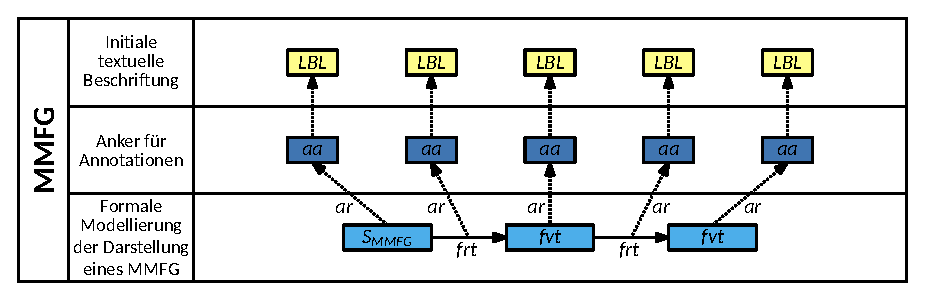
\includegraphics[width=\textwidth]{chapter/chapter_2/mmfg/annotation/formal-model-syntactic-mmfg-incl-annotations.eps}
    \caption{Formale Modellierung der Darstellung eines MMFG inkl. Anker für Annotationen.}
    \label{sec2:sota:subsec:fz-explainablity:fig:mmfg-formal-model-mmfg-incl-annotations}
\end{figure}
In \cref{sec2:sota:subsec:fz-explainablity:fig:mmfg-formal-model-mmfg-incl-annotations} ist in einer zweiten Ebene \enquote{Anker für Annotationen} die formale Darstellung von Annotationsankern zu sehen.
Diese Anker sind Knoten, die dem MMFG hinzugefügt werden und über eine neue Beziehung $ar$ mit jedem Knoten oder jeder Kante im ursprünglichen MMFG verbunden werden können.
Die dritte Ebene führt eine Variable $LBL$ ein, um eine klare Differenzierung zwischen Merkmalen und der textuellen Darstellung dieser Merkmale zu schaffen und ermöglicht eine für Menschen verständliche textuelle Darstellung von Merkmalen.

Diese Erweiterungen ermöglichen das Anbinden von Elementen eines MMFGs an Elemente von bestehenden semantischen Darstellungen und ihren entsprechenden für Maschinen lesbaren Darstellungen im Semantic Web.
Die Darstellung semantischer Informationen wird durch die vom W3C herausgegebenen Standards des Semantic Webs abgedeckt.
Die Grundlage für diese Darstellungen und Annotationen ist für gewöhnlich ein an einem Bereich orientiertes Vokabular.
Sobald Beziehungen zwischen den Begriffen dieses Vokabulars eingeführt werden, können Taxonomien gebildet werden, welche bereits definierte textuelle Bezeichnungen und Synonyme enhalten.
Mittels Taxonomien können diese Begriffe dann nach bestimmten Kriterien klassifiziert und in Kategorien oder Klassen eingeordnet werden.
In einem weiteren Schritt können Ontologien die Beziehungen zwischen Begriffen einer Taxonomie beschreiben und so über die hierarchische Struktur von Taxonomien hinweggreifen.
Das Resource Description Framework (RDF) dient als Grundlage zur Beschreibung jeglicher Art von Informationen im Semantic Web durch den Einsatz eines Extensible Markup Language (XML) Syntaxs.
Da RDF auf XML basiert, kann es in Form eines Graphen dargestellt und auf die Struktur eines MMFGs abgebildet werden.

Anbindung vom Semantic Web im GMAF ansprechen (SemWebExtension)
RDF-Beispiel?
Dann Übergang zur Erweiterung von Grammatik um zusätzliche Elemente

\cref{sec2:sota:subsec:fz-explainablity:fig:mmfg-formal-schema-mmfg-ex-incl-annotation} zeigt die Erweiterung des $MMFG_{ex}$ um die neuen Elemente $aa$ und $ar$.

\begin{figure}[htb]
    \centering
    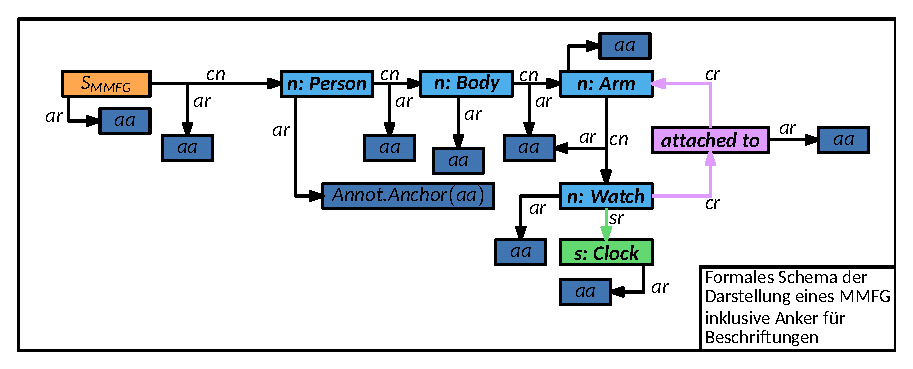
\includegraphics[width=\textwidth]{chapter/chapter_2/mmfg/annotation/formal-schema-mmfg-ex-incl-annotation.eps}
    \caption{Formales Schema der Darstellung des $MMFG_{ex}$ inkl. Anker für Annotationen.}
    \label{sec2:sota:subsec:fz-explainablity:fig:mmfg-formal-schema-mmfg-ex-incl-annotation}
\end{figure}

Um formale Ausdrücke mitsamt Annotationsanker konstruieren zu können, muss die Grammatik $G_{MMFG}$ ebenfalls um die neuen Elemente $aa$ und $ar$ erweitert werden.
Das Erweitern der Grammatik erfolgt durch das Hinzufügen der Elemente $aa$ und $ar$ in die Menge $N_{MMFG} = FVT_{MMFG} \cup FRT_{MMFG} \cup \{aa, ar\}$, sowie durch eine Anpassung der Produktionsregeln wie folgt:
\setlength{\s}{\widthof{$S_{MMFG} \hspace*{\widthof{$FVT_{MMFG}$} - \widthof{$S_{MMFG}$}}\rightarrow FVT_{MMFG}~FRT_{MMFG}~FVT_{MMFG}$}}
\setlength{\p}{\widthof{$P_{MMFG} = \{$}}
\newlength{\fvt}
\setlength{\fvt}{\widthof{$FVT_{MMFG}$} - \widthof{$ar$}}
\allowdisplaybreaks
\begin{align*}
    %\begin{split}
            P_{MMFG} = \{ \hspace*{\s + 0.1cm} \\
            S_{MMFG} \hspace*{\widthof{$FVT_{MMFG}$} - \widthof{$S_{MMFG}$}}\rightarrow FVT_{MMFG}~FRT_{MMFG}~FVT_{MMFG} \\
            FVT_{MMFG} \rightarrow ar \hspace*{\s - \widthof{$FVT_{MMFG} \rightarrow ar$}} \\
            FRT_{MMFG} \rightarrow ar \hspace*{\s - \widthof{$FRT_{MMFG} \rightarrow ar$}} \\
            ar \rightarrow aa \hspace*{\s - \widthof{$FRT_{MMFG} \rightarrow ar$}} \\
            aa \rightarrow LBL \hspace*{\s - \widthof{$FRT_{MMFG} \rightarrow LBL$}} \\
            \} \hspace{\s}
    %\end{split}
\end{align*}
Anhand dieser Anpassungen können nun Ausdrücke wie: 
\newline
\enquote{person is-annotated-with-the-semantic-concept rdf:person has-child-is-annotated-with-the-semantic-concept rdf:related body is-annotated-with-the-semantic-concept rdf:head}.
?Überleitung zu semantischer Annotation...

\paragraph{Semantische Annotation der formalen Darstellung von MMFGs}
\label{sec2:sota:par:semantic-annot-formal-representation-smmfgs}
Die Erweiterung der formalen Darstellung von MMFGs um Annotationsanker $aa$ und entsprechender Beziehung $ar$ stellt eine reine strukturelle Erweiterung eines MMGs dar.
Diese Struktur muss nachwievor mit semantischen Darstellungen annotiert werden.
Hierfür muss eine weitere Erweiterung der formalen Darstellung eines MMFG um folgende Elemente vorgenommen werden:
\begin{itemize}
    \item Einen Knoten zur semantischen Darstellung (engl. \textit{semantic node representation $(snr)$}) für jeden Knoten in einem MMFG, sowie einen weiteren Knoten zur semantischen Darstellung von Beziehungen (engl. \textit{semantic relationship representation $(srr)$}) für jede Kante bzw. Beziehung in einem MMFG.
    Diese Elemente sind essentiell zur semantischen Darstellung von Bedeutungen von Knoten und Kanten in einem MMFG.
    \item Eine Menge $SFVT_{MMFG}$ und $SRVT_{MMFG}$.
    Während in einem MMFG die Mengen $FVT_{MMFG}$ und $FRT_{MMFG}$ die Bezeichnungen von Merkmale bzw. der Beziehungstypen darstellen, stellen nun in einem SMMFG die Mengen $SFVT_{MMFG}$ und $SRVT_{MMFG}$ die Bedeutungen dieser Bezeichnungen bzw. Beziehungstypen dar.
    Somit wird jede Bezeichnung $fvt_i \in FVT_{MMFG}$ durch einen semantischen Begriff $sfvt_i \in SFVT_{MMFG}$ dargestellt.
    Analog wird jeder Beziehungstyp $frt_i \in FRT_{MMFG}$ durch einen semantischen Begriff $srvt_i \in SRVT_{MMFG}$ dargestellt.
    \item Die Beziehungen in einem MMFG werden in einer formalen Darstellung nur durch ihre Typen (z.B. cn, t, sr) dargestellt.
    Diese Typen werden in einem SMMFG nun durch semantische Begriffe $srvt_i \in SRVT_{MMFG}$ modelliert. 
    Die Menge $SRVT_{MMFG}$ stellt somit die Bedeutung der Begriffe dar, die die Beziehungen in einem MMFG beschreiben.
    \item In einem MMFG ist jeder Knoten und jede Kante durch eine Annotationsbeziehung $ar$ mit einem Annotationsanker verbunden.
    Diese Annotationsanker werden nun durch die Knoten $snr$ und $srr$ dargestellt.
    Ein Annotationsanker $aa$ stellt im Endeffekt einen Uniform Resource Identifier (URI) 
    für den verbundenen Knoten oder die verbundene Kante dar.
    Sinn und Zweck eines Annotationsankers ist es somit die Knoten oder Kanten eines MMFGs mit einem Knoten $snr$ zur semantischen Darstellung eines Begriffs oder einem Knoten $srr$ zur semantischen Darstellung einer Beziehung miteinander zu verbinden.
    \item Die Beziehung $hasName$ in einem SMMFG verbindet einen Knoten zur semantischen Darstellung eines Begriffs mit einem Begriff $sfvt_i \in SFVT_{MMFG}$ und analog einen Knoten zur semantischen Darstellung einer Beziehung mit einem Begriff $srvt_i \in SRVT_{MMFG}$.
    Jeder Knoten $srr$ zur semantischen Darstellung einer Beziehung verweist mit jeweils zwei Beziehungen $domain$ und $range$ zu entsprechenden Knoten $snr$.
    Die Beziehung $domain$ verweist auf den Startknoten zur semantischen Darstellung eines Begriffs und die Beziehung $range$ auf den Endknoten zur semantischen Darstellung eines Begriffs.
\end{itemize}
Durch diese Erweiterung wird ein MMFG zu einem semantisch annotierten MMFG bzw. zu einem semantischen MMFG (SMMFG).
\cref{sec2:sota:subsec:fz-explainablity:fig:mmfg-formal-model-smmfg} zeigt wie durch die Knoten $snr$ und $srr$ Annotationsanker mit semantischen Begriffen aus den Mengen $SFVT_{MMFG}$ und $SRVT_{MMFG}$ verbunden werden können.
Zusammen mit den Beziehungen zwischen den semantischen Darstellungen der Struktur eines MMFGs, wie z.B den Beziehungen $domain$ und $range$ zwischen den entsprechenden $snr$ Knoten, bilden diese die semantische Annotation der ersten Ebene und folglich einem semantisch annotierten MMFG bzw. SMMFG.
Die semantische Annotation der zweiten Ebene erfolgt durch die Begriffe $sfvt_i \in SFVT_{MMFG}$ und $srvt_i \in SRVT_{MMFG}$, welche die Bedeutung der Bezeichungen von Merkmalen darstellt. 

\begin{figure}[htb]
    \centering
    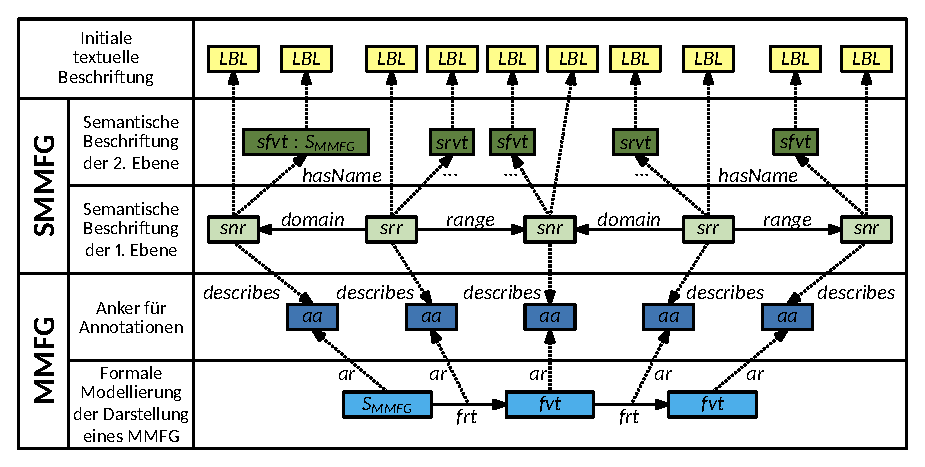
\includegraphics[width=\textwidth]{chapter/chapter_2/mmfg/semantic/formal-model-syntactic-smmfg.eps}
    \caption{Formale Modellierung der Darstellung eines SMMFG.}
    \label{sec2:sota:subsec:fz-explainablity:fig:mmfg-formal-model-smmfg}
\end{figure}
Sollen aus einem SMMFG zulässige formale Ausdrücke generiert werden, so muss die Grammatik $G_{MMFG}$ anhand dieser Erweiterungen um die neuen Elemente des SMMFG erweitert werden.
Das Erweitern dieser Grammatik führt zu einer neuen Grammatik $G_{SMMFG} = (N_{SMMFG},~\Sigma_{SMMFG},~P_{SMMFG},~S_{SMMFG}=S_{MMFG})$ zur Konstruktion zulässiger formaler Ausdrücke aus einem SMMFG.
Folgende Erweiterung müssen vorgenommen werden:
\begin{itemize}
    \item $N_{SMMFG} = N_{MMFG} \cup SNR \cup SRR \cup SFVT_{SMMFG} \cup SRVT_{SMMFG}$ ist die neue Menge der semantischen Darstellungen von Bezeichnungen von identifizierten Merkmalen und Beziehungen in einem MMFG.
    \item $\Sigma_{SMMFG}$ ist eine Erweiterung der Menge $\Sigma_{MMFG}$ um die neuen semantischen Beziehungen der Bezeichnungen
\end{itemize}

\begin{figure}[htb]
    \centering
    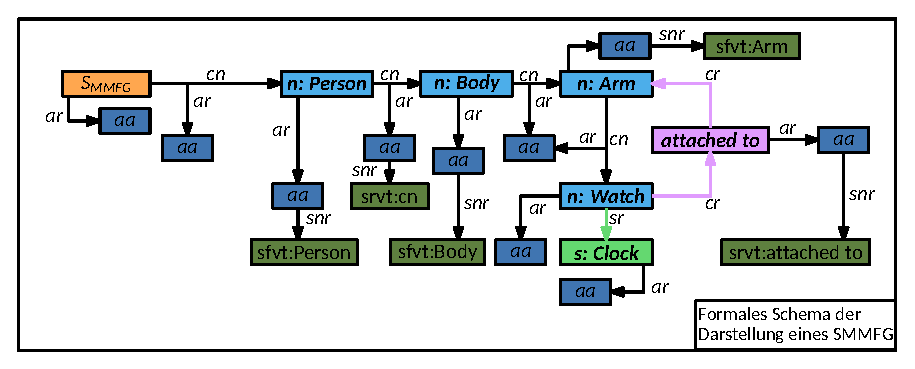
\includegraphics[width=\textwidth]{chapter/chapter_2/mmfg/semantic/formal-schema-smmfg-ex.eps}
    \caption{Formales Schema der Darstellung des $SMMFG_{ex}$.}
    \label{sec2:sota:subsec:fz-explainablity:fig:mmfg-formal-schema-smmfg}
\end{figure}

\paragraph{Erklärbare Semantische MMFGs (ESMMFGs)}
\label{sec2:sota:par:explainable-smmfgs}

\begin{figure}[htb]
    \centering
    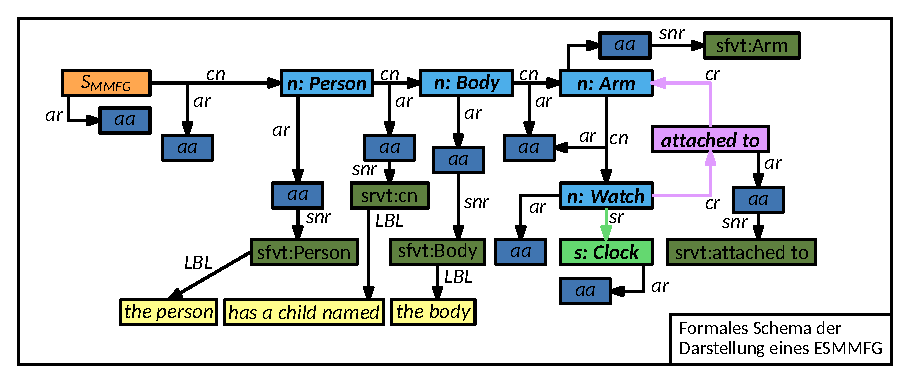
\includegraphics[width=\textwidth]{chapter/chapter_2/mmfg/explainable/formal-schema-esmmfg-ex.eps}
    \caption{Formales Schema der Darstellung des $ESMMFG_{ex}$.}
    \label{sec2:sota:subsec:fz-explainablity:fig:mmfg-formal-schema-esmmfg}
\end{figure}

\begin{figure}[htb]
    \centering
    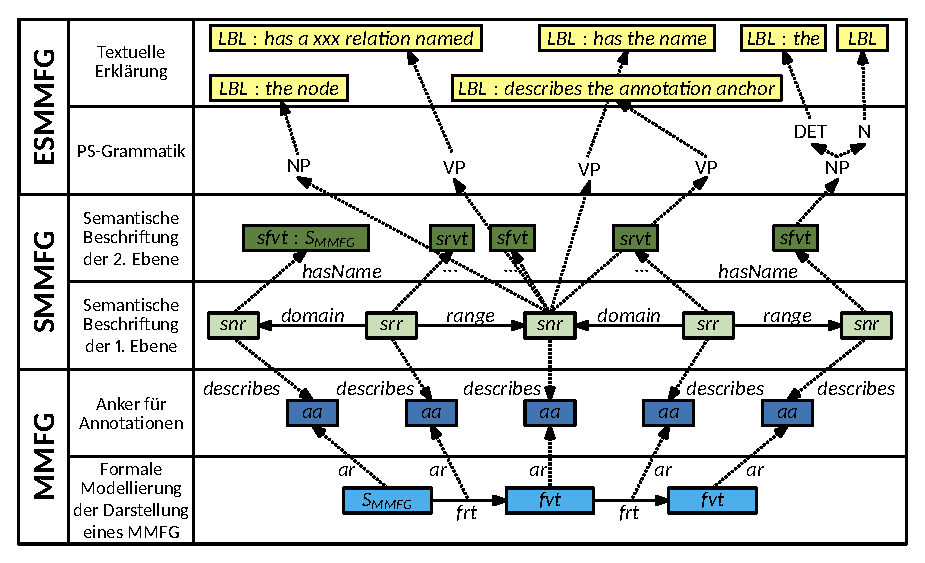
\includegraphics[width=\textwidth]{chapter/chapter_2/mmfg/explainable/formal-model-syntactic-esmmfg.eps}
    \caption{Formale Modellierung der Darstellung eines ESMMFG.}
    \label{sec2:sota:subsec:fz-explainablity:fig:mmfg-formal-model-esmmfg}
\end{figure}